
%%%%%%%%%%%%%%%%%%%%%%%%%%%%%%%%%%%%
%%%%%%%%%%%%%%%%%%%%%%%%%%%%%%%%%%%%
%%%%%%%%%%%%%%%%%%%%%%%%%%%%%%%%%%%%
\section{Derived GSQL operators over GSM}
The previous section constructively provided the basic building blocks for expressing data operations. The present section will show that those 
%The previous section described the basic building blocks that 
can be used to express all the possible operations on top of GSMs.
In particular, we will
%The current section shows that, after representing each data model in GSM as already stated in the previous chapter, we can 
 redefine all the source models' usual operators and provide traversal semantics. We first describe  set operators  (Subsection \vref{ssec:gsmsop}) and then we extend them to relational and semistructured operators (Subsection \vref{ssec:gsmrelop}). %Afterwards, we will show that the combination of the former with the following GSQL operators allows the expression of queries of practical interest, from traversal queries to nested graph ones.
These operators are going to introduce the nesting operator, which is going to express abstraction, grouping and $\otimes_\theta$-products (as well as joins).
%definition of both XPath traversal and graph traversal operations (Subsection \vref{ssec:travgraphop}), and last we're going to show how such algebra is also able to express operators over (nested) graphs (Subsection \vref{ssec:ngrahop}).

%%%%%%%%%%%%%%%%%%%%%%%%%%%%%%%%%%%%
%%%%%%%%%%%%%%%%%%%%%%%%%%%%%%%%%%%%
%%%%%%%%%%%%%%%%%%%%%%%%%%%%%%%%%%%%
\subsection{(Attribute labelled) Set operations}\label{ssec:gsmsop}
In this section we're going to define set operations using the disjoint union operator combined to a \texttt{map}, given that \texttt{map} can represent most of the unary operators. Consequently, for all the binary (or $n$-ary) set operations, we must use \texttt{disjoint} first and then transform the elements. Each binary (or $n$-ary) is going to be carried out over  each operand's reference object. The set operations are going to be carried out over the collections' referenced by the same expression $p$ via $\phi(o_i,p)$ for each $1\leq i\leq n$.
% the containment associated to both operands referenced by the same attribute. 

Please note that in the following definitions we're going to omit the \texttt{script} syntax in favour of a more compact mathematical notation. Nevertheless, we're going to provide the script definition of the incoming $\psi$ functions in Appendix \vref{app:scriptnote}.

We now introduce the first GSQL set operation, that is the union. 
We must remark that this operator is anyway different from the traditional union operator defined for sets: while the present operator considers that two element are the same if and only if they are indeed the same object, the set operator considers two elements to be equivalent just if they have the same value. This consideration implies that some relational algebra operators can be defined through the definition of an equivalence predicate between the objects, and thus requiring the definition of the ``group by'' operator, that we are going to provide in the next subsection.


\begin{definition}[Union]\label{def:gsmunion}
	\index{GSQL!$\bigcup$}
	Given $n$ GSMs  $n^i=(o_c^i,O,\ell^i,\xi^i,\phi^i)$ for each $1\leq i\leq n$, their \textbf{union} $\bigcup_{1\leq i\leq n}n^i$ maps the union of their object into a new reference object $\omega$, where only the resulting reference object is transformed as follows:
	\[\psi_\cup=o\mapsto p\mapsto\bigcup_{1\leq i\leq n}\phi_{n^1\dots n^n}(\omega,[i,p])\]
	Therefore, the result of the union will return a reference object containing either the union of the containments associated to the same attribute $p$ in both operands, or their preservation. The operator can be defined as follows:
	\[\bigcup_{1\leq i\leq n}^\omega n^i=\texttt{map}_{\ell_{n^1\dots n^n},\xi_{n^1\dots n^n},\phi_{n^1\dots n^n}\oplus \psi_\cup}(\texttt{disjoint}^\omega(n^1,\dots,n^n))\]
\end{definition}

We can define the intersection and difference operators similarly to the union as follows:
\begin{definition}[Intersection]
	\index{GSQL!$\bigcap$}
	Given $n$ GSMs  $n^i=(o_c^i,O^i,\ell^i,\xi^i,\phi^i)$ for each $1\leq i\leq n$, their \textbf{intersection} $\bigcap_{1\leq i\leq n}n^i$ maps the intersection of their object into a new reference object $\omega$, where only the reference object is transformed in the $\phi$ function as follows:
	\[\psi_\cap=o\mapsto p\mapsto\bigcap_{1\leq i\leq n}\phi_{n^1\dots n^n}(\omega,[i,p])\]
	Therefore, the result of the intersection will return a reference object containing the intersection of the containments associated to the same attribute $p$ in both operands. The operator can be defined as follows:
	\[\bigcap_{1\leq i\leq n}^\omega n^i=\texttt{map}_{\ell_{n^1\dots n^n},\xi_{n^1\dots n^n},\phi_{n^1\dots n^n}\oplus \psi_\cap}(\texttt{disjoint}^\omega(n^1,\dots,n^n))\]
\end{definition}

\begin{definition}[Difference]
	\index{GSQL!$\backslash$}
	Given two GSMs  $n=(o_c,O,\ell,\xi,\phi)$ and $n'=(o'_c,O',\ell',\xi',\phi')$, their \textbf{difference} $n\backslash^\omega n'$ maps the union of their object into a new reference object $\omega$, where only the reference object is transformed in the $\phi$ function as follows:
	\[\psi_\backslash=o\mapsto p\mapsto \phi_{n,n'}(\omega, [1,p])\backslash\phi_{n,n'}(\omega, [2,p])\]
	Therefore, the result of the intersection will return a reference object containing the intersection of the containments associated to the same attribute $p$ in both operands, and the remaining elements from the sole left operand:
	\[n\backslash^\omega n'=\texttt{map}_{\ell_{nn'},\xi_{nn'},\phi_{nn'}\oplus \psi_\cap}(\texttt{disjoint}^\omega(n,n'))\]
\end{definition}

\begin{figure}[!t]
	\centering
	\begin{minipage}[t]{0.9\textwidth}
		\centering
		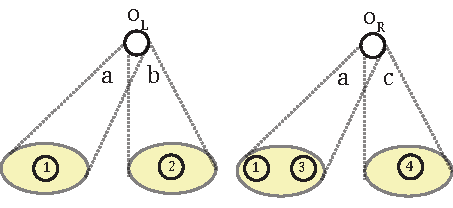
\includegraphics[scale=0.8]{fig/05language/03setop_operands.pdf}
		\subcaption{Two possible operands for the set operations. Even in this case, $o_L$ is the reference object for the GSM $n^L$, while $o_R$ is the reference object for $n^R$.}
		\label{fig:setoperands}
	\end{minipage}
	\begin{minipage}[t]{0.3\textwidth}
		\centering
		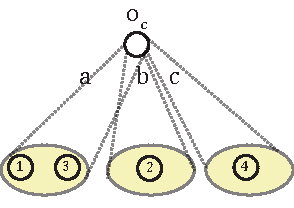
\includegraphics[scale=0.8]{fig/05language/04setop_union.pdf}
		\subcaption{$n^L\cup n^R:=\bigcup\{n^L,n^R\}$}
		\label{fig:setunion}
	\end{minipage}\begin{minipage}[t]{0.3\textwidth}
	\centering
	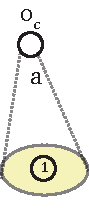
\includegraphics[scale=0.8]{fig/05language/06setop_intersection.pdf}
	\subcaption{$n^L\cap n^R:=\bigcap\{n^L,n^R\}$}
	\label{fig:setintersection}
\end{minipage}\begin{minipage}[t]{0.1\textwidth}
	\centering
	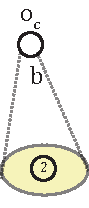
\includegraphics[scale=0.8]{fig/05language/05setop_difference.pdf}
	\subcaption{$n^L\backslash n^R$}
	\label{fig:setdifference}
\end{minipage}
	\caption{Representing different possible outcomes for the set operators. While the \texttt{disjoint} operator treated each operand's containment as an element of a set represented by the object itself, these operations treat each containment as a collection. Moreover, the set operations are carried out over the set sharing the same labels.}
	\label{fig:setoperations}
\end{figure}


\begin{example}
This example provides some graphical representations of the former multi-set operations. Let us take a look at Figure \vref{fig:setoperations}: set operations are performed over the containments both at the collection level (the set operation is performed over all the collections identified by the same attribute) and at the object level. While the union operation (\subref{fig:setunion}) merges the collections with the same attribute (containments) coming from both operands, the intersection (\subref{fig:setintersection}) keeps only the ones appearing in both operands and, while doing so, it preserves only the object shared between the collections. Last, the difference (\subref{fig:setdifference}) keeps only those collections (containments) appearing on the left operand ($n^L$) and, among those collections, only the element not appearing in the attribute-correspondent collection in $n^R$ are preserved.
\end{example}

Given that $\phi$ associates to each object $o$ the attributes $p$ alongside their list of values $\phi(o,p)$, we can slightly change the previous operations in order to define the combine operation required for the relational join operation, as already outlined in Definition \vref{def:concatenation}. As a consequence, even the combine operator may be expressed as the following derived operator.

\begin{definition}[Object Concatenation]
	Given two GSMs  $n$ and $n'$, their \textbf{concatenation}\index{GSQL!$\oplus$} $n\oplus n'$ maps them into a new reference object $\omega$, such that the attribute-values coming from the first operand are rewritten in favour of the ones coming from the second operand when sharing the same attribute. Therefore, the operator is defined as follows:
	\[n\oplus^\omega n'=n'\cup^\omega (n\backslash n')\]
	%is the GSM associated to a new object ${\tilde o}_{c}$
	%which $id$ is defined as $\tilde{o}=\max\{\max_{o}{o_c\in O},\max_{o'}o'_c\in O'\}+1$. Such object has the labels and expressions associated to both $o$ and $o'$, while the collections associated via $\phi$ and existing in both $o_c$ and $o'_c$ are replaced by the ones in $o'_c$.
	%\begin{alignat*}{2}
	%n\oplus n'=(&\tilde{o}_c,\\
	%            &O\cup O'\cup\{\tilde{o}_c\},\\
	%            &\ell\oplus \ell'\oplus[\tilde{o}_c\mapsto \ell(o_c)\cup\ell'(o'_c)]\\
	%            &\xi\oplus\xi'\oplus[\tilde{o}_c\mapsto \xi(o_c)\cup\xi'(o'_c)]\\
	%            &\phi\oplus\phi'\oplus [\tilde{o}_c\mapsto \psi_1)]\\
	%\end{alignat*}
	%In particular, the $\oplus$ was already defined for functions at page \pageref{sec:tautonesting}, and $\psi_1$ is defined as follows:
	%\[\psi_1(p)=\begin{cases}
	%	\phi'(o'_c,p) & p\in\dom(\phi'(o'_c))\\
	%	\phi(o_c,p)  & \textup{oth.}\\
	%\end{cases}\]
\end{definition}

The former operation shows that the MOF objects and sets are uniformely represented within this data model through GSM reference objects: this is evident from the definition of the object concatenation operator, which was defined through the composition of over set operators.
